\documentclass{article}

\usepackage{graphicx}
\usepackage[hidelinks]{hyperref}
\usepackage[a4paper, total={6in, 8in}]{geometry}
\usepackage[slovak]{babel}
\usepackage{caption}
\usepackage{subcaption}

\graphicspath{./include/}

\renewcommand{\figurename}{Obr.}
\renewcommand{\contentsname}{Obsah}

\begin{document}

\begin{titlepage}
	\null\vfill

	\begin{center}
		{\Huge Meranie a aproximácia prevodovej charakteristiky tepelného systému }
		\vskip 2cm

		{\Large Cvičenie č. 11}
		\vskip 0.5cm

		{\large Spojité procesy}
	\end{center}

	\vfill
	\vfill

	\begin{flushright}
		Filip Lobpreis \\
		Matúš Machata \\
		\small\today\\
	\end{flushright}
	\hfill
\end{titlepage}

\thispagestyle{empty}
\clearpage

\tableofcontents
\thispagestyle{empty}
\clearpage

\section{Zadanie}
\label{sec:zadanie}
\pagenumbering{arabic}

\begin{figure}[!htbp]
	\begin{center}
		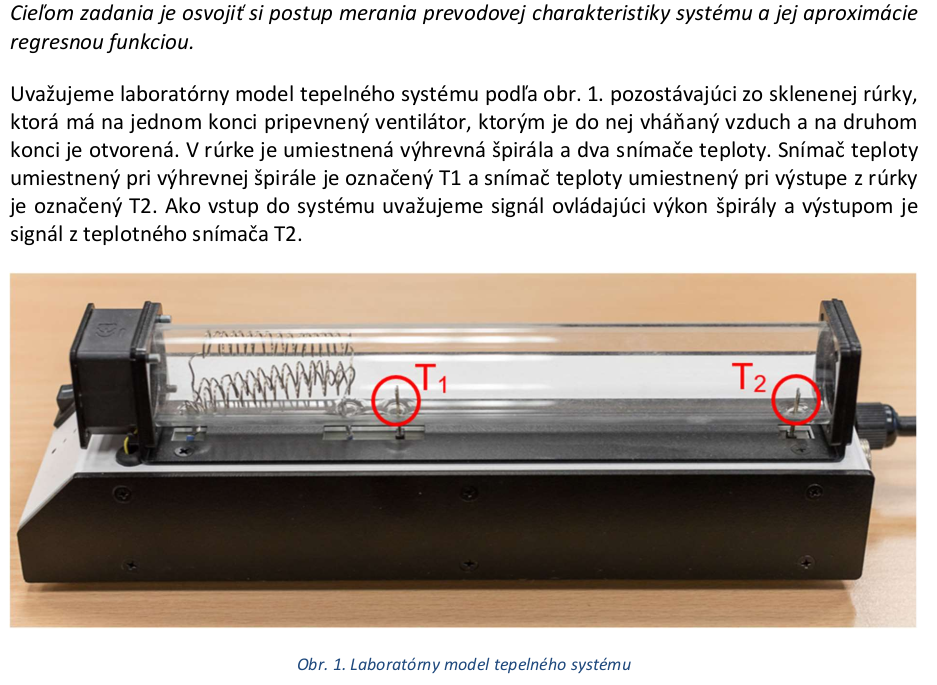
\includegraphics[width=0.8\textwidth]{./include/zadanie.png}
	\end{center}
	\caption{Prvá časť zadania z~cvičenia č. 11 z~predmetu spojité procesy}
	\label{fig:zadanie1}
\end{figure}

\clearpage

\section{Teória}
\label{sec:teoria}

V~tomto zadaní je našou úlohou experimentálne overiť návrh regulácie výšky hladiny na~laboratórnom
modeli tepelného systému a~overiť navrhované riešenie. Pri~tomto zadaní sme použili už~preddefinovanú schému
v~programe \textit{Simulink} (Obr.~\ref{fig:schema}).

\begin{figure}[!htbp]
	\begin{center}
		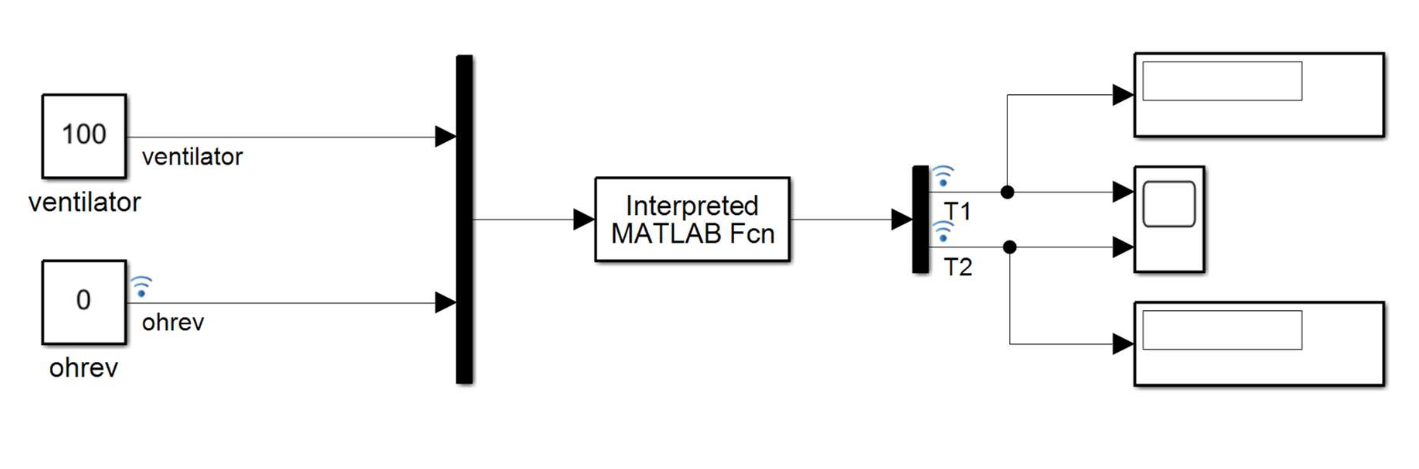
\includegraphics[width=0.8\textwidth]{./include/schema.png}
	\end{center}
	\caption{Schéma modelu z~cvičenia č. 11 z~predmetu spojité procesy}
	\label{fig:schema}
\end{figure}

V~tomto zapojení vidíme viacero vstupných signálov, tie sú už~preddefinované. \textbf{ventilator} reprezentuje na kolko percent funguje ventilator v systeme. \textbf{ohrev} reprezentuje vstupny signal ohrevnej spiraly, jeho hodnoty
sú zadávané v~percentách. Tuto hodnotu budeme v priebeju merania prestavovoat. Bude sa menit od 0\% po 100\% s krokom 10\%.

\clearpage

\subsection{Úvod do~priebehu simulácie}
\label{subsec:priebehSimulacie}

Počas priebehu simulácie sa spomínaná žiadaná hodnota výšky hladiny mení. Priebeh zmien tejto veličiny je znázornený na~obrázku Obr.~\ref{fig:mt2}.
Na zaciatku merania sme nastavili ohrev spiraly na 10\%. Postupne sme zvyšovali hodnotu ohrevu až k~100\%.
Kedze sme prvu hodnotu nenastavili na 0\%, tak sme meranie zopakovali. Pri druhom merani sme dostali hodnoty,
ktore boli vyssie ako hodnoty z prveho merania. Pri aproximácia budeme pouzivat hodnoty z druhej casti merania.

\begin{figure}[!htbp]
	\begin{center}
		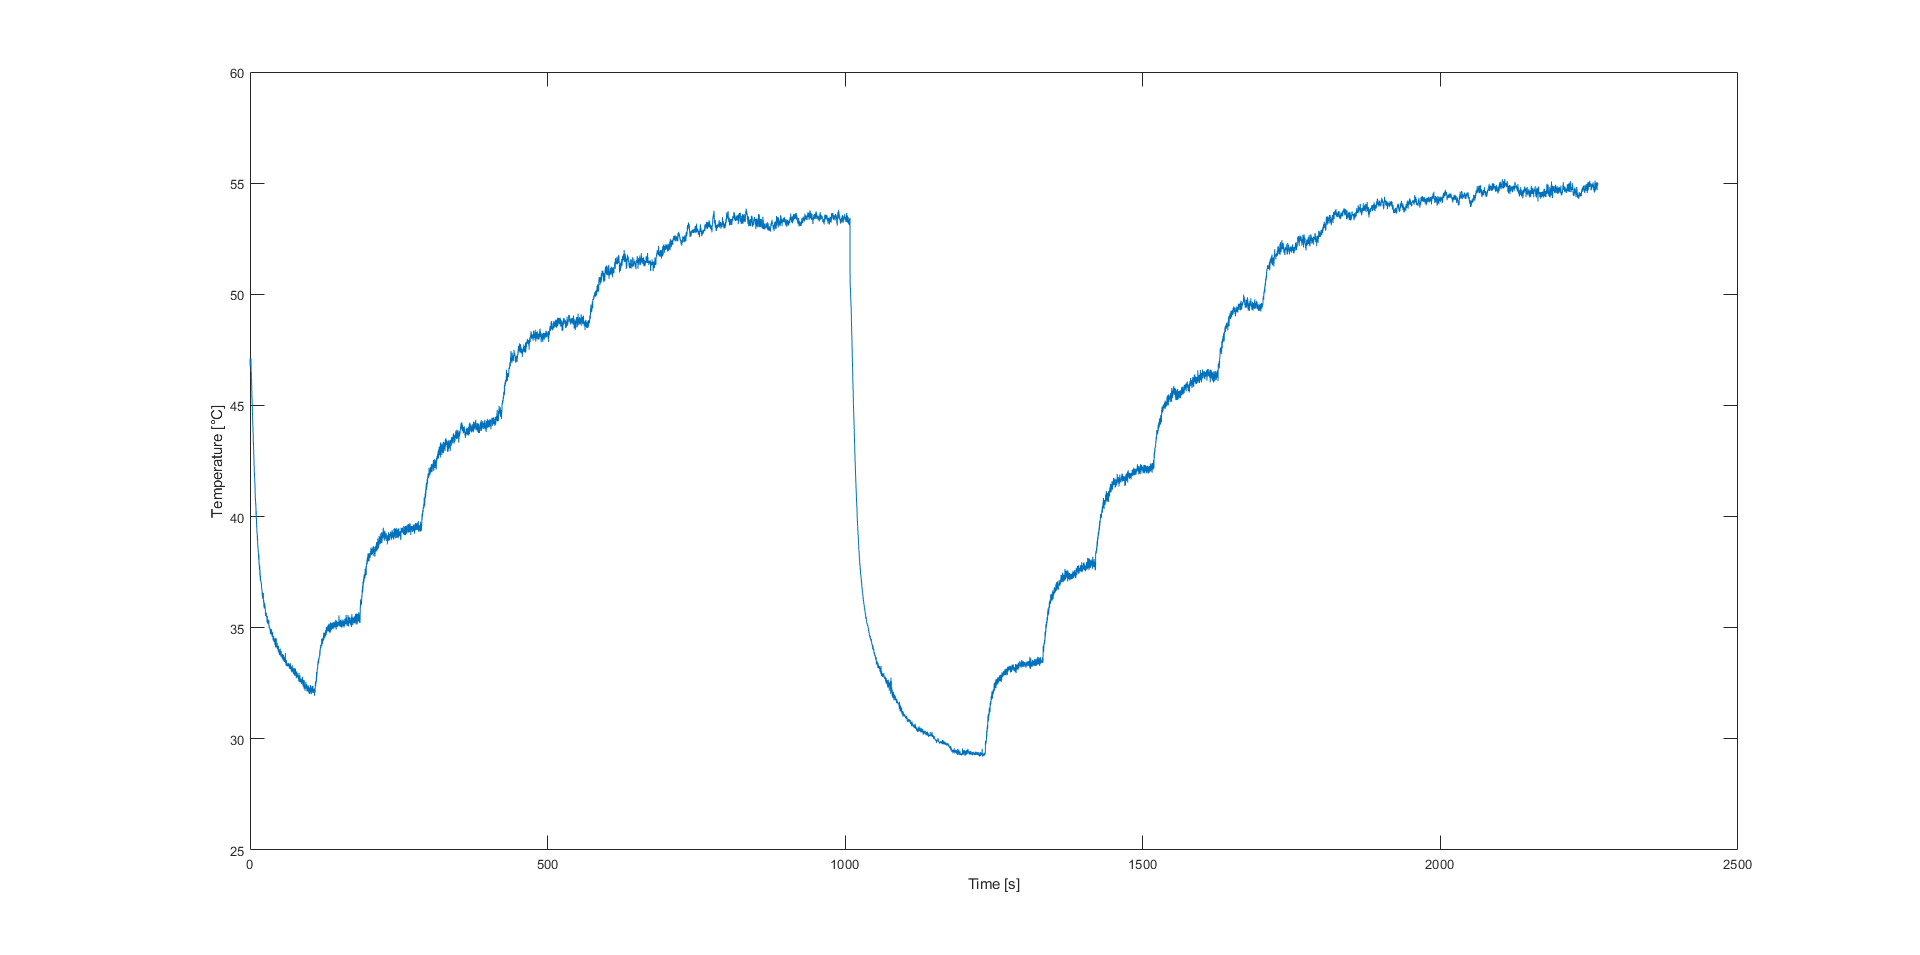
\includegraphics[width=\textwidth]{./include/teplota.png}
		\caption{Priebeh meranej teploty na snímači T2.}
		\label{fig:mt2}
	\end{center}
	\hfill
\end{figure}

Merane hodnoty nam vysli nasledovne:

\begin{center}
\begin{tabular}{ |c|c|c| }
 \hline
 ohrev [\%] & T1 [$^\circ $C] & T2 [$^\circ $C] \\
 \hline
   0 & 29.3 & 29 \\
  10 & 33.5 & 33 \\
  20 & 38 & 37 \\
  30 & 42 & 41\\
  40 & 46.5 & 45\\
  50 & 49.5 & 47.5\\
  60 & 52.5 & 50 \\
  70 & 54 & 51.3 \\
  80 & 54.5 & 51.6 \\
  90 & 55 & 52 \\
 100 & 55 & 52 \\
 \hline
\end{tabular}
\end{center}
\newpage

\section{Meranie}
\label{sec:meranie}

\clearpage

\section{Linearna aproximacia}
\label{sec:lin}

Pri lineárnej aproximácii sme potrebovali vytvoriť maticu H, vypočítať \(\theta\) pomocou Gaussovím vzťahom \(\theta = (H^TH)^-1H^Ty\), následne sme si pomocou vzťahu \(y_1 = H_1\theta_1\) vyjadrili funkciu opisujúcu fukciu pre výstupné veličiny. Hodnoty účelovej funkcie sme si vypočítali zo vzťahu \(Q1 = e^Te\). Na Obr.~\ref{fig:prevod} môžeme vidieť porovnanie prevodových funkcii s lineárnou aproximáciou.

\clearpage

\section{Kvadraticka aproximacia}
\label{sec:kvad}

\clearpage

\section{Odmocninova aproximacia}
\label{sec:odm}

\clearpage



\section{Zhrnutie}
\label{sec:zhrnutie}

\begin{figure}[!htbp]
	\begin{center}
		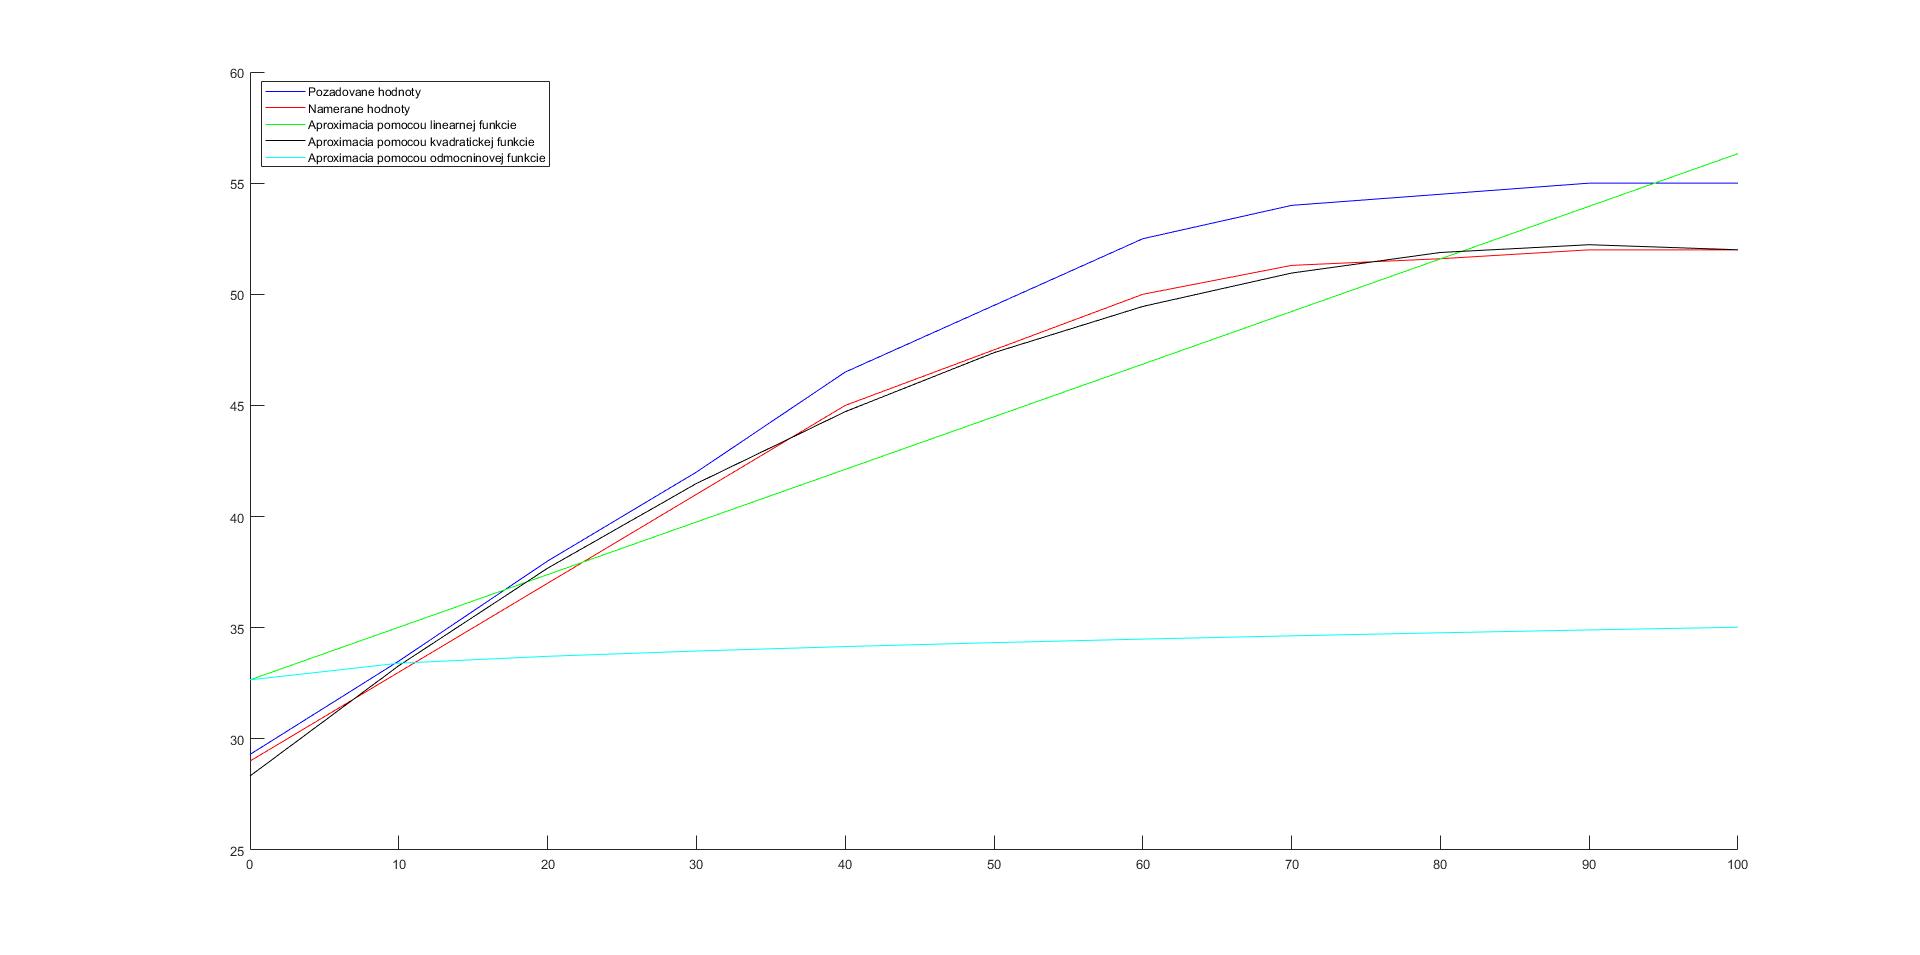
\includegraphics[width=\textwidth]{./include/prevodove_funkcie.png}
		\caption{Priebeh prevodových funkcii}
		\label{fig:prevod}
	\end{center}
	\hfill
\end{figure}


\end{document}

